\chapter{Pruebas del sistema}
\label{pruebas}

\section{Funcionamiento del sistema}
\subsection{SolarGraficos}
\subsubsection{Información general de la estación}
\begin{figure}[h]
	\centering
	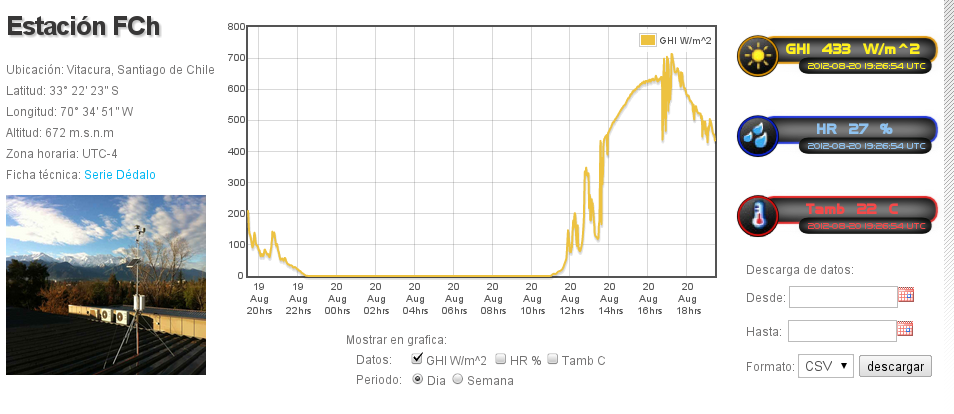
\includegraphics[scale=0.42]{./images/cap5chap1img0}
	\caption{Presentación de la aplicación}
	\label{graficoPresentacion}
\end{figure}
A la izquierda, en la primera columna (Ver. Fig. \ref{graficoPresentacion}), la aplicación muestra la información general de la estación, presentando datos tales como: nombre, ubicación política y geográfica, altitud, zona horaria donde se encuentra y finalmente una ficha técnica sobre el hardware que posee. En la parte inferior se puede apreciar una fotografía de esta.

\begin{figure}[h]
	\begin{minipage}[b]{0.45\linewidth}
		\centering
		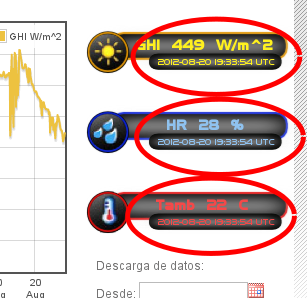
\includegraphics[scale=0.5]{./images/cap5chap1img5-1}
		\caption{Primera marca}
		\label{primeraMarca}
	\end{minipage}
	\begin{minipage}[b]{0.45\linewidth}
		\centering
                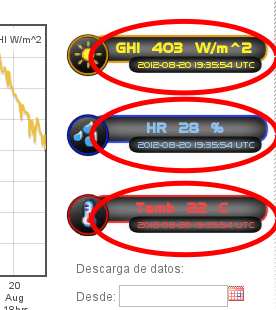
\includegraphics[scale=0.5]{./images/cap5chap1img5-2}
                \caption{Segunda marca}
                \label{segundaMarca}
	\end{minipage}
\end{figure}
En la columna derecha de la aplicación, se presentan indicadores de la ultima medición obtenida (Ver. Fig. \ref{primeraMarca} y \ref{segundaMarca}). Por cada parámetro que la estación mide, hay un ''widget'' que muestra el valor numérico de la medición junto a sus unidades y nombre. En la zona inferior de cada medición se muestra la fecha a la que se asocia dicha medición.

\subsubsection{Manejo del visualizador}
\begin{figure}[ht]
        \centering
        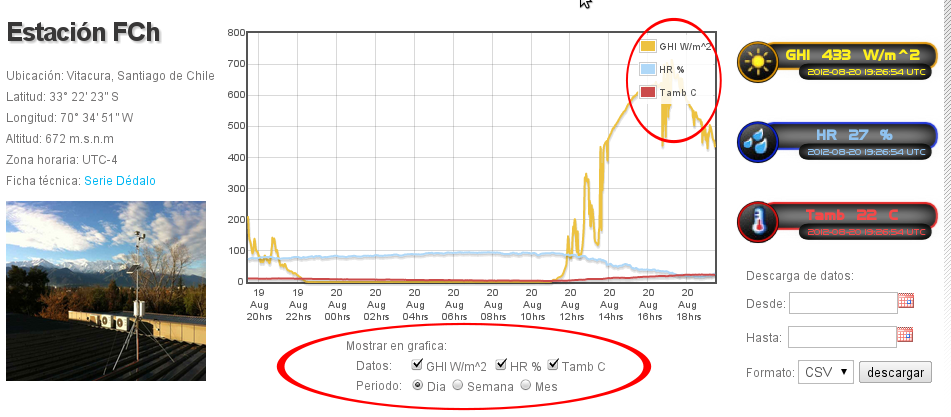
\includegraphics[scale=0.4]{./images/cap5chap1img1}
        \caption{Visualizador - Curvas de la gráfica}
        \label{visualizador}
\end{figure}
La primera herramienta de la cual dispone ''solarGraficos'', da la posibilidad de habilitar o deshabilitar en la gráfica las curvas para los diferentes parámetros medidos por la estación, estas pueden mostrarse de manera individual o bien en conjunto (ver Fig: \ref{visualizador}).

\begin{figure}[ht]
        \centering
        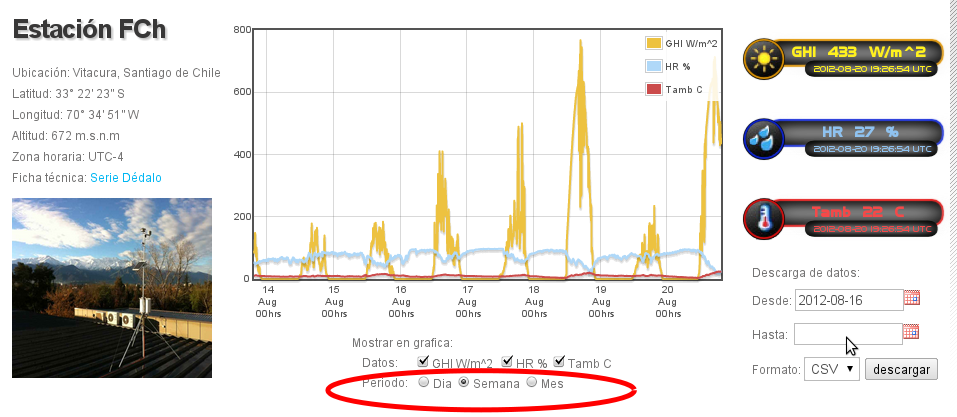
\includegraphics[scale=0.4]{./images/cap5chap1img3}
        \caption{Visualizador - Periodos de tiempo}
        \label{visualizadorTiempo}
\end{figure}
Siguiendo con las herramientas de configuración de la gráfica, la figura \ref{visualizadorTiempo} nos muestra la posibilidad de modificar los periodos de tiempo que se muestran para cada una de las curvas, dado que la cantidad de datos con la que se dibujan las gráficas son bastante grandes, estas toma algún tiempo en cargarse, por lo que si observamos con mas detalle, las opciones para mostrar las curvas en periodos de una semana, un mes o un año, irán apareciendo a medida que los datos estén totalmente cargados. Esta carga ocurre de manera trasparente, por lo que mientras esto sucede el usuario puede hacer uso de todas las demás funcionalidades de la aplicación.\\

Para obtener mas detalles respecto de alguna medición en particular reflejada en la gráfica, basta con posicionar el cursor sobre la curva deseada y esta identificara de manera automática los puntos donde exista una medición, marcando el punto con un circulo a su alrededor, adicionalmente mostrara una pequeña ventana emergente con información detallada de la medición, unidades, hora y fecha especifica. La figura \ref{cursor} muestran como esta característica se aplica a cada una de las curvas.

\begin{figure}[ht]
	\begin{minipage}[b]{0.32\linewidth}
        	\centering
        	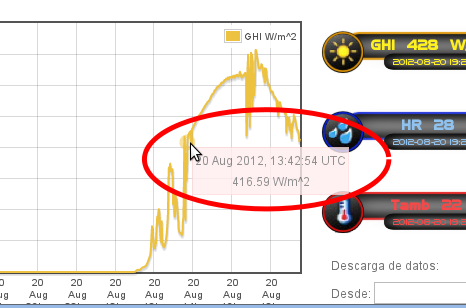
\includegraphics[scale=0.35]{./images/cap5chap1img4-1}
	\end{minipage}
	\begin{minipage}[b]{0.32\linewidth}
                \centering
                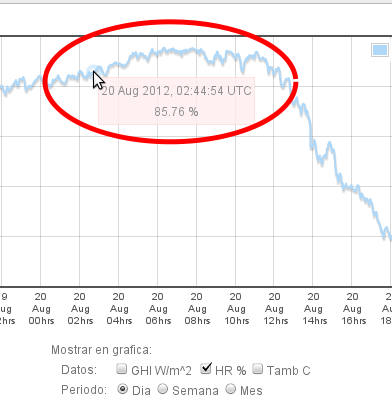
\includegraphics[scale=0.35]{./images/cap5chap1img4-2}
        \end{minipage}
	\begin{minipage}[b]{0.32\linewidth}
                \centering
                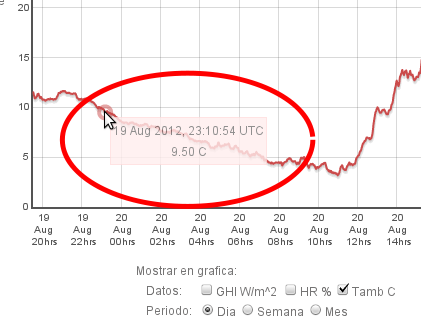
\includegraphics[scale=0.35]{./images/cap5chap1img4-3}
        \end{minipage}
	\caption{Posición del cursor}
	\label{cursor}
\end{figure}

\newpage
\subsubsection{Descarga de datos}
La aplicación cuenta con un módulo que permite descargar los datos directamente desde el ''Servidor de almacenamiento de datos'', de forma personalizada, para ello, en la sección inferior derecha, bajo el titulo ''Descarga de datos'' hay dos campos denominados ''desde'' y ''hasta'', al hacer clic en cada uno de ellos se despliega un calendario que permite seleccionar el día específico para cada campo (Ver. Fig. \ref{calendario}). Mediante esta utilidad podemos especificar el rango de tiempo que contendrá el fichero descargado con los datos en formato CSV. Este fichero puede ser utilizado en diversas aplicaciones externas para cargar los datos y realizar cualquier tipo de procesamiento deseado (Ver. Fig. \ref{descargafichero}).

\begin{figure}[ht]
	\begin{minipage}[b]{0.47\linewidth}
        	\centering
        	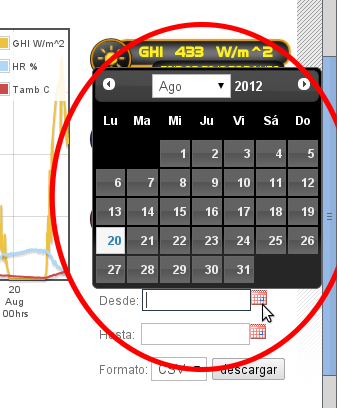
\includegraphics[scale=0.5]{./images/cap5chap1img2-1}
	\end{minipage}
	\begin{minipage}[b]{0.47\linewidth}
	 	\centering
        	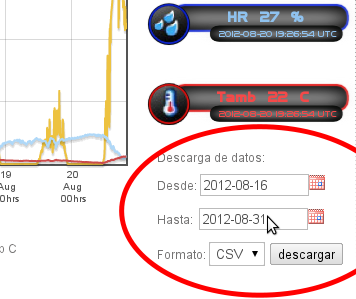
\includegraphics[scale=0.5]{./images/cap5chap1img2-2}
	\end{minipage}
	\caption{Descarga de datos - Calendario}
	\label{calendario}
\end{figure}

\begin{figure}[ht]
	\centering
        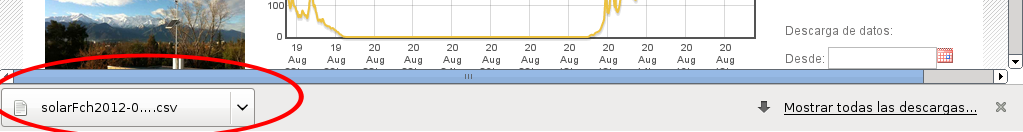
\includegraphics[scale=0.45]{./images/cap5chap1img2-3}
        \label{descargafichero}
	\caption{Descarga de datos - Fichero}
\end{figure}

\newpage 
\subsection{SolarCalc}
\subsubsection{Presentación inicial}
\begin{figure}[ht]
        \centering
        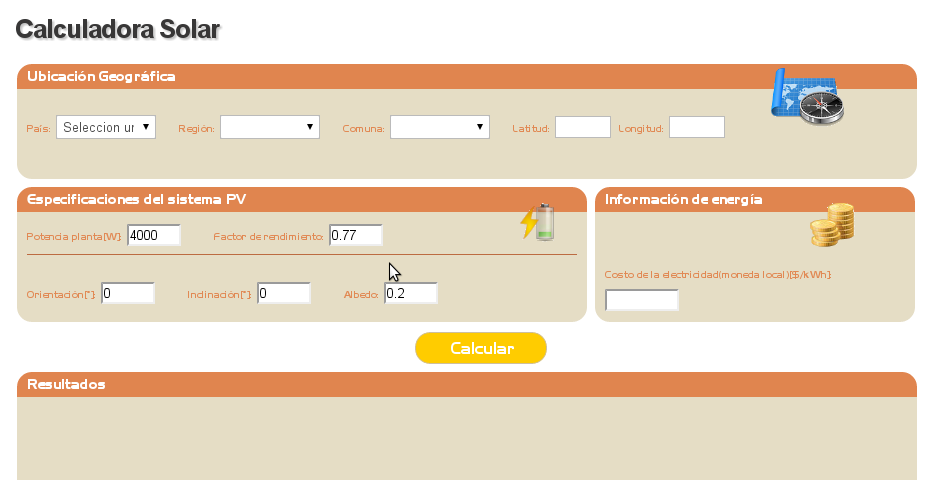
\includegraphics[scale=0.4]{./images/cap5chap1img6}
        \caption{Presentación Calculadora}
        \label{figCalculadora}
\end{figure}

Al cargar la calculadora se aprecia la figura \ref{figCalculadora}, adaptada a los requerimientos planteados, es una interfaz sencilla, con la menor cantidad de parámetros necesarios, los cuales se van actualizando a medida que el usuario los rellena. Dividida en 4 secciones de acuerdo a la caracterización de los parámetros.

\subsubsection{Ubicación geográfica}
La primera sección que se debe rellenar es la posición geográfica donde se pretende instalar la planta a simular, por el momento la calculadora solo cuenta con información de Chile (Ver. Fig. \ref{pais}) en todas sus Regiones y Comunas.\\ Al momento de seleccionar la comuna (Ver. Fig. \ref{region}), el sistema automáticamente establece las coordenadas geográficas del centro de esta. Como indica la figura, los parámetros deben ser ingresados en orden secuencial, iniciando por el país, luego la región y finalmente la comuna, de manera de permitir al sistema ir cargando la información de forma dinámica.
\begin{figure}[ht]
	\centering
	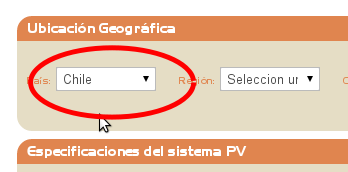
\includegraphics[scale=0.5]{./images/cap5chap1img7-1}
	\caption{País}
	\label{pais}
\end{figure}

\begin{figure}[ht]
	\centering
	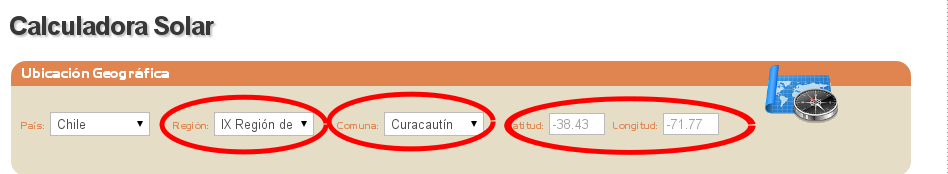
\includegraphics[scale=0.5]{./images/cap5chap1img7-2}
	\caption{Región, comuna, coordenadas geográficas}
	\label{region}
\end{figure}

\subsubsection{Especificaciones del sistema PV e información de la energía}
Esta sección es una de las mas complejas si no se cuenta con cierto conocimiento técnico de los sistemas fotovoltaicos, acá se debe proporcionar a la calculadora parámetros específicos (Ver Fig:\ref{sistemaPv}) de la configuración de los equipos de la planta a simular.\\

\begin{figure}[h]
        \centering
        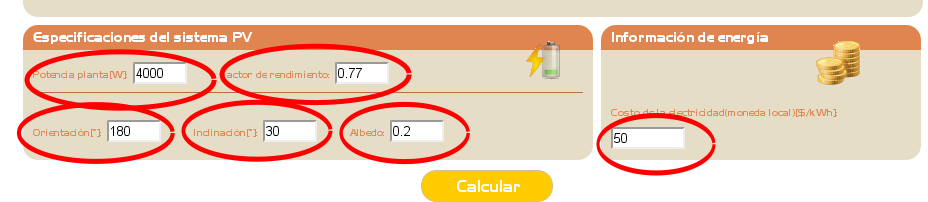
\includegraphics[scale=0.4]{./images/cap5chap1img8}
        \caption{Especificación del sistema PV}
        \label{sistemaPv}
\end{figure}

\paragraph{Potencia de la planta:} Es la suma de la potencia individual de cada uno de los módulos fotovoltaicos del sistema, la que se puede encontrar en la etiqueta trasera de estos.\\
Como referencia, un módulo PV de 1,5[m] de alto por 1[m] de ancho (1,5[m2]) de Silicio policristalino, produce 200[W] de Potencia bajo STC (“Standard Test Conditions” asume 1000[W/m2] de radiación solar, una temperatura ambiente de $25^\circ C$ y velocidad del viento de 1[m/s]).\\ Una instalación de 4000[W] corresponde a 30 [m2] de superficie cubierta con módulos solares.
 
\paragraph{Factor de rendimiento:} Factor que incorpora las pérdidas respecto al proceso completo de conversión de energía, desde que sale de los paneles hasta que está disponible en corriente alterna, respecto a la situación ideal sin pérdidas. Su valor típico es 0.77, variando según el sistema entre 0.62 y 0.96.\\
Consiste en la multiplicación de los factores asociados a pérdidas en los cables, conexiones y diodos, eficiencia del inversor y transformador, variación respecto al valor de placa del módulo solar, entre otros.

\paragraph{Orientación:} Corresponde a la orientación de los paneles respecto al punto cardinal Norte, en la figura expresado por el ángulo $\alpha$ en grados.\\Si el panel se encuentra orientado hacia el Norte, corresponde a $0\circ$, aumentando a medida que se gira hacia el Sur, en sentido horario (Oeste=$270\circ$, Sur=$180\circ$, Este=$90\circ$).

\paragraph{Inclinación:} Corresponde a la inclinación de los paneles respecto al eje horizontal, en la figura expresado por el ángulo $\beta$ en grados.

\begin{figure}[h]
        \centering
        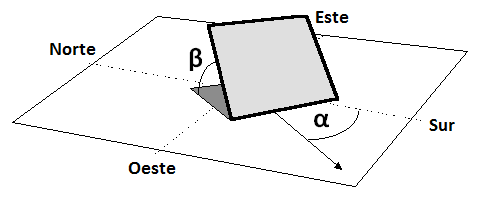
\includegraphics[scale=0.5]{./images/planoPanelSolar}
        \caption{Orientación del sistema PV}
        \label{orientacionSistemaPV}
\end{figure}

\paragraph{Albedo:} Índice sobre el porcentaje de radiación que una superficie refleja, respecto a la que recibe. Mientras mayor es el índice, más radiación refleja. Para el suelo común y corriente se considera 0.2, y para el concreto 0.5, mientras que para la nieve sería 0.85.

\paragraph{Costo de la energía:} Precio que se paga en la moneda local, por cada kWh consumido en el lugar de la instalación.
Generalmente sale expresado en la factura de electricidad.

\subsubsection{Resultados}
Finalmente, luego de llenar toda la información solicitada, se debe hacer clic en el botón ''calcular'', pasados unos segundos el sistema entregara un resultado dividido en 3 sección principales (Ver Fig:\ref{resultadosCalc}). La primera sección es una tabla de resultados la cual nos informa mes a mes para un año típico, la cantidad de radiación media, la cantidad de energía producida específicamente para los parámetros de configuración ingresados y el costo de venta que debiese tener la energía producida, este ultimo paramentar representa una utilidad en cuanto si se desea utilizar estos cálculos en alguna propuesta económica para la instalación de alguna planta.\\ La según sección nos muestra, en la parte inferior izquierda, un gráfico anual en el tiempo y dos ejes laterales, este gráfico nos informa respecto de la eficiencia que tendrá el sistema PV comparando la curva de radiación con la curva de energía producida.\\ Finalmente el gráfico de la para inferior derecha tiene como objetivo caracterizar la radiación solar en un año meteorológico típico para cada mes, con la cual se realizaron los cálculos.

\begin{figure}[h]
        \centering
        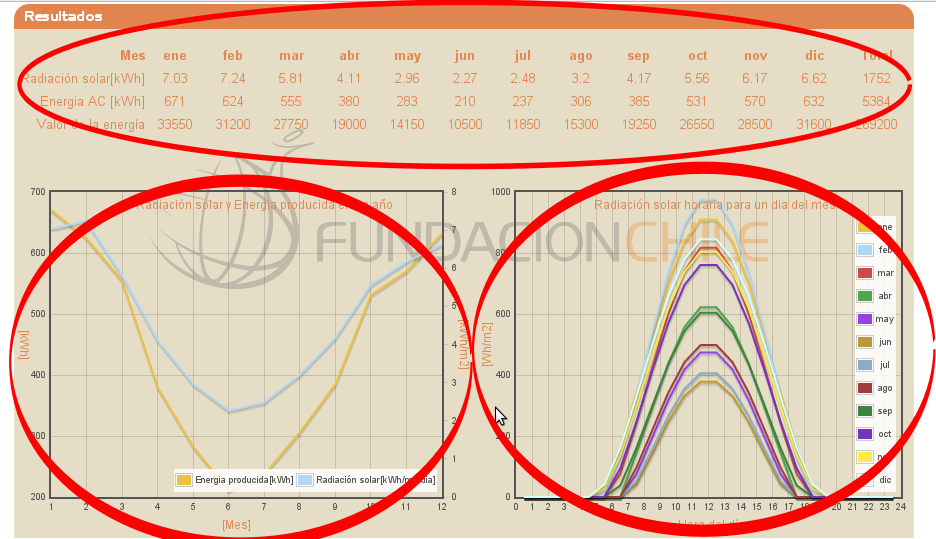
\includegraphics[scale=0.4]{./images/cap5chap1img9}
        \caption{Resultados de la Calculadora}
        \label{resultadosCalc}
\end{figure}

\newpage
\section{Pruebas de comunicación}
Uno de los problemas más complejos que se enfrentó durante el desarrollo de esta Memoria fue el diseño e implementación de los sistemas de comunicación, que permitieron establecer conexiones confiables y seguras entre las distintas componentes del sistema. De acuerdo al diseño planteado en el capítulo \ref{solucion}, se puede apreciar que la comunicación entre la componente de ''Aplicaciones'' y la de ''Almacenamiento de datos'' fue más o menos trivial, dentro de lo que se refiere a la comunicación Web en un sistema informático, sin embargo, al momento de interconectar las ''Estaciones de medición'' con el resto del sistema hubo que considerar muchas variables extras, tales como: geográficas, ambientales y eléctricas.\\

Las estaciones, al estar ubicadas en lugares geográficos remotos, en la mayoría de los casos no disponen de cables o conexiones a la red de datos. La señal de telefonía celular con buen soporte de datos no es de buena calidad en todos los lugares del país y con menor razón en lugares como el Desierto de Atacama, en medio de cordones montañosos e incluso en lugares más aislados. Las estaciones, según requerimientos, debían disponer de un sistema de comunicación flexible, que pudiese ser adaptado a todas las condiciones y dificultades anteriormente mencionadas, para esto se diseño un sistema, de forma que permitiese adaptar diferentes tecnologías, sin embargo, para efectos prácticos de esta Memoria, se implementaron dos módulos diferentes: Comunicación a través de Ethernet y comunicación vía módem de telefonía celular.

\subsection{Caso de Pruebas}
En las próximas secciones de este capitulo se exponen diferentes pruebas realizadas al sistema, entre ellas, la conectividad con las estaciones de medición, los servidores de datos y aplicaciones. Además se realizaron pruebas para verificar los métodos de calculo, la programación y la correctitud de los resultados teóricos en comparación con resultados empíricos. Para las pruebas de comunicación se utilizo una estación Dédalo (Ver Anexo \ref{dedalo}), denominada en capítulos anteriores como ''Estación Fch'' la cual es la estación ubicada en las dependencias de Fundación Chile en la comuna de Vitacura de la Región Metropolitana. Esta estación durante el periodo de prueba midió: Radiación solar global en el plano horizontal, Temperatura ambiente y humedad relativa del aire. Además se considera el periodo de prueba como el funcionamiento normal entre las fechas de Mayo del 2012 y Septiembre 2012, considerando de forma especial una interrupción programada en el mes de Agosto para mantención de los instrumentos, por el periodo de una semana y 6 interrupciones no programadas por fallos en la conectividad del sistema inferiores a 6 horas de funcionamiento cada una, producto del funcionamiento defectuoso de una batería de la estación, lo cual dejo a esta, sin electricidad en dichas ventanas de tiempo, una vez diagnosticado el problema se procedió a reemplazar la batería defectuosa solucionando así el problema.\\
Para la comparación teórica de los cálculos, se utilizaron bases de datos elaboradas por ''PVWatts'', considerando muestras de un año meteorológico típico para la comunas de Vitacura, Antofagasta y Concepción.  
 
\subsection{Comunicación de estación ''VitacuraFCh'' con ''Servidor de datos'' - Vía Ethernet}
Una de las primeras actividades que se realizó en esta Memoria, fue la interiorización con los equipos que componen las estaciones meteorológicas, esto involucró el aprender a utilizar elementos de hardware tales como el ''datalogger'' Campbell Scientific CR1000, módems de telefonía celular y otras interfaces de comunicación.\\
Para lograr que la estación se comunique de forma autónoma con el ''Servidor de almacenamiento de datos'' fue necesario escribir un programa para el ''datalogger'' que fuese capaz de realizar una petición GET a través del módulo ''Campbell NL200'', utilizando la implementación del protocolo TCP/IP de esta Interfaz. Para esto, fue necesario conectar el módulo ''NL200'' a través de la interfaz ''SCI/O'' del ''datalogger'' y configurar el módulo para actuar en modo ''bridge'', esto permite una comunicación transparente, entre el ''datalogger'' y la red informática de Fundación Chile.

Esta modalidad del sistema de comunicación es bastante limitada, ya que es necesario contar en los lugares de instalación de las estaciones con una infraestructura de red de datos informática.

Para verificar el estado de la conexión, se exponen dos métodos, en primer lugar la conexión manual utilizando el software proporcionado por el fabricante ''PC400'', a través de este software establecemos una conexión ''TCP/IP'', utilizando la dirección IP asignada a la estación y realizamos una prueba de descarga de datos:

\begin{enumerate}
\item Ejecutar el PC400
\item Creamos una nueva conexión (Ver Fig:\ref{ether1}) 
\item En la sección ''comunication setup'', seleccionamos el dispositivo ''CR1000'' y luego seleccionamos el tipo de convección ''Ip Port''.
\item Ingresamos la dirección IP de la estación y finalizamos la configuración (Ver Fig:\ref{ether2}).
\item En la pantalla principal, en el menú de la izquierda seleccionamos la nueva interfaz y presionamos el botón ''connect'' (Ver Fig:\ref{ether3})
\item Una vez establecida la conexión, vamos a la solapa superior que dice ''monitor data'' y podemos observar los parámetros que la estación esta midiendo (Ver Fig:\ref{ether4}).
\item Finalmente vamos a la solapa ''collect data'', presionamos en ''collect'' y esperamos a que se complete la descarga (Ver Fig:\ref{ether5}).
\end{enumerate}

\begin{figure}[h!]
        \centering
        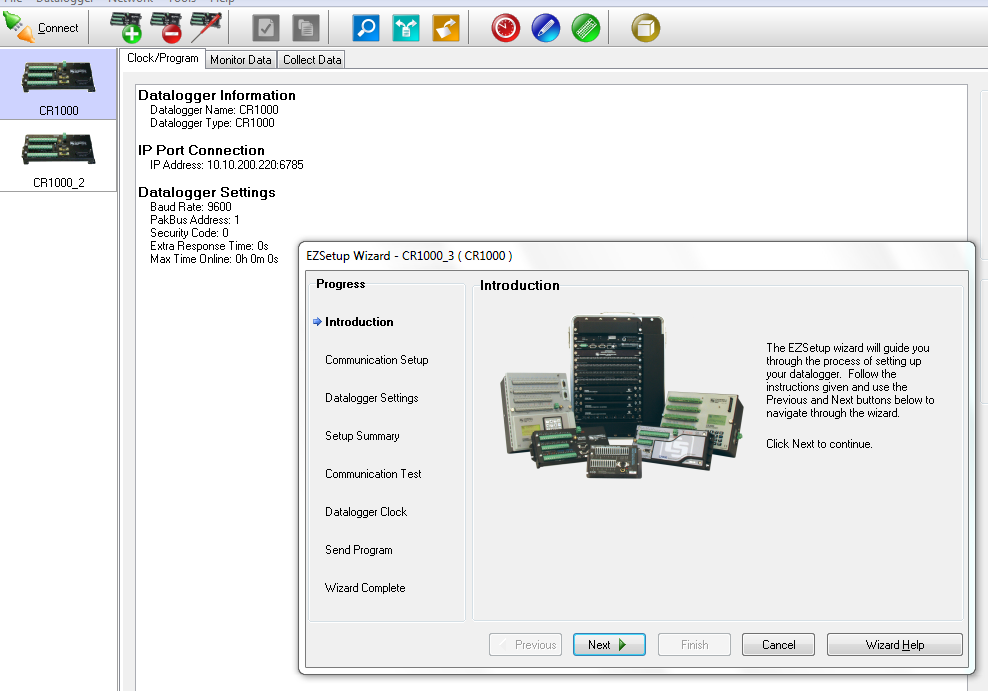
\includegraphics[width=320pt]{images/pruebas1}
        \caption{Crear nueva conexión}
        \label{ether1}
\end{figure}
\begin{figure}[h!]
        \centering
        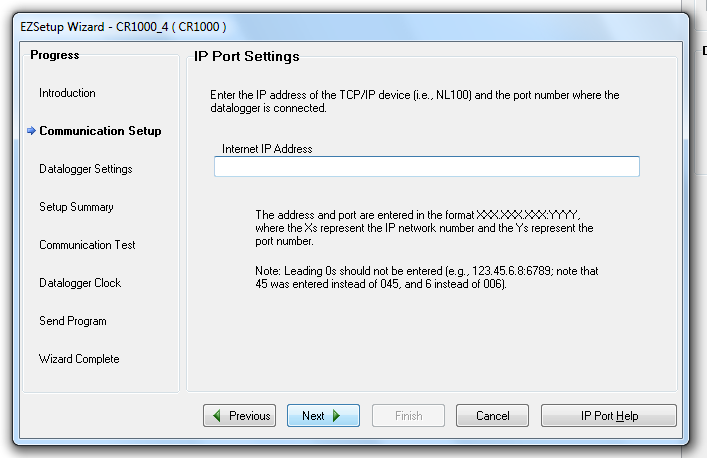
\includegraphics[width=400pt]{images/pruebas2}
        \caption{Ingresar dirección IP}
        \label{ether2}
\end{figure}

\newpage
\begin{figure}[h!]
        \centering
        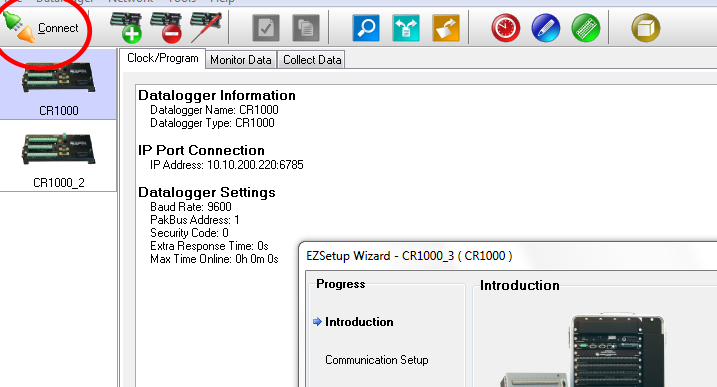
\includegraphics[width=400pt]{images/pruebas3}
        \caption{Estableciendo conexión}
        \label{ether3}
\end{figure}
\begin{figure}[h!]
        \centering
        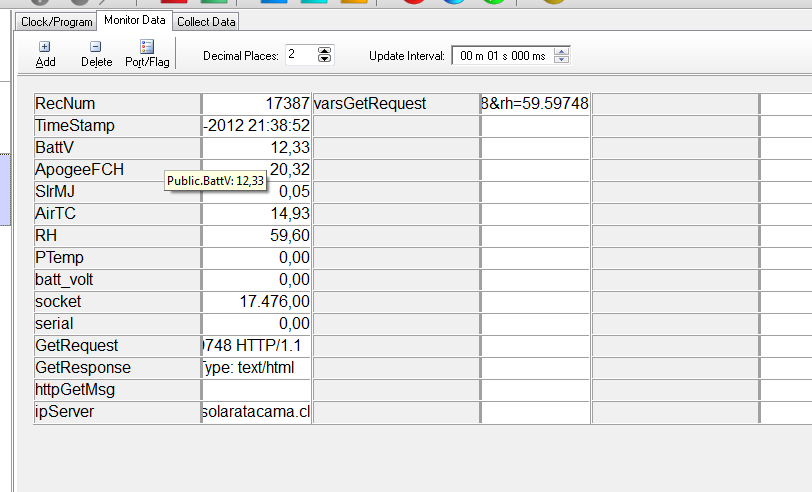
\includegraphics[width=400pt]{images/pruebas4}
        \caption{Monitorizar datos de estación}
        \label{ether4}
\end{figure}

\newpage
\begin{figure}[h!]
        \centering
        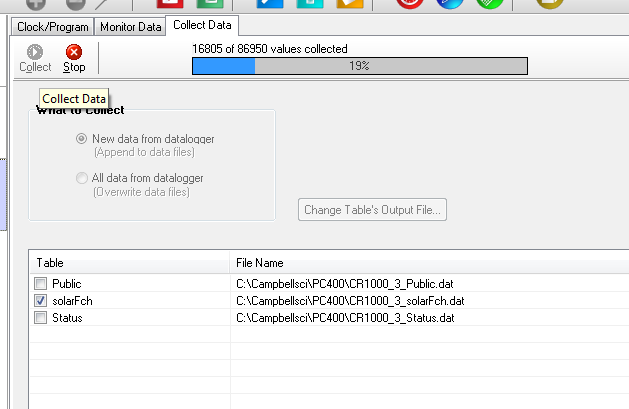
\includegraphics[width=400pt]{images/pruebas5}
        \caption{Descarga de datos}
        \label{ether5}
\end{figure}

\subsection{Comunicación de las estación ''VitacuraFch'' con el ''Servidor de datos''}
Para verificar la conexión autónoma desde la estación hacia la red se presenta el registro del servidor Web Apache HTTPD cuando la estación realiza la petición GET (Ver Fig:\ref{pruebasLog1}).

\begin{figure}[h!]
        \centering
        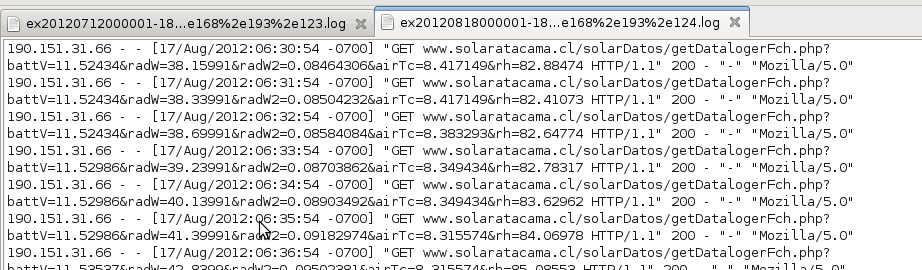
\includegraphics[width=400pt]{images/pruebasLog1}
        \caption{Logs Apache HTTPD - Comunicación con estación meteorológica}
        \label{pruebasLog1}
\end{figure}

\subsection{Comunicación de estación ''VitacuraFCh'' con ''Servidor de datos'' - Vía Módem telefonía celular}
Este tipo de comunicación, es el segundo método que se implementó en esta Memoria y en comparación al método anterior es mucho mas flexible, ya que es posible establecer comunicación con estaciones de forma inalámbrica en diferentes ubicaciones de la geografía nacional, incluso en lugares remotos. Actualmente el desarrollo de esta tecnología en nuestro país, permite establecer comunicación en lugares bastante remotos como sectores montañosos en la cordillera o bien en medio del Desierto de Atacama.\\

Para testear la comunicación mediante este modulo se utiliza el software proporcionado por el fabricante del ''datalogger'', el ''PC400'' siguiendo los siguientes pasos:

\begin{enumerate}
\item Ejecutar el PC400
\item Creamos una nueva conexión (Ver Fig:\ref{ether1})
\item En la sección ''comunication setup'', seleccionamos el dispositivo ''CR800'' y luego seleccionamos el tipo de conexión ''Phone Modem'' (Ver Fig:\ref{modem1}) y luego la opción ''Use módem from CSI list'' (Ver Fig:\ref{modem2}).
\item Seleccionamos el puerto COM donde esta conectado el módem (Ver Fig:\ref{modem3}) y en la lista siguiente, seleccionamos el modelo del miden que vamos a utilizar, Para este caso particular fue necesario configurar un nuevo módem).
\subitem Para configurar un nuevo módem, hacemos clic en ''Edit Modem Database'' (Ver Fig:\ref{modem4}), luego bajo la lista que hay en la nueva ventana desplegada hacemos clic en ''New'', ingresamos el nombre del nuevo módem y presionamos ''OK''
\subitem Finalmente editamos los parámetros del nuevo módem. ''Reset strng'' lo seteamos en blanco e ''Initialization String'' lo dejamos en \textbf{\&C0\&D0}, luego hacemos clic en ''Save'' (Ver Fig:\ref{modem5}). 
\item Una vez configurado el módem, ingresamos el ''Phone Number'', numero de teléfono que tienen el módem al cual vamos a llamar y presionamos en ''Next'' para ir al siguiente paso.
\item En esta nueva ventana configuramos el ''Baud Rate'' en \textbf{9600} y Finalizamos la configuración.
\item Finalmente hacemos clic en el botón superior izquierdo con la nueva conexión seleccionada para abrir un canal de comunicación con la estación.
\item Una vez establecida la conexión vamos a la solapa superior que dice ''monitor data'' y podemos observar los parámetros que la estación esta midiendo (Ver Fig:\ref{ether4}).
\item Finalmente vamos a la solapa ''collect data'', presionamos en ''collect'' y esperamos a que se complete la descarga (Ver Fig:\ref{ether5}).
\end{enumerate}
\begin{figure}[h!]
        \centering
        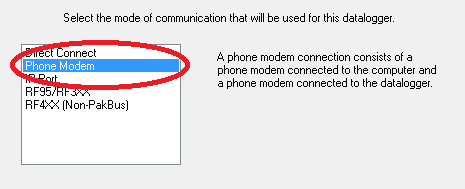
\includegraphics[width=320pt]{images/modem1}
        \caption{Seleccionar módem}
        \label{modem1}
\end{figure}
\begin{figure}[h!]
        \centering
        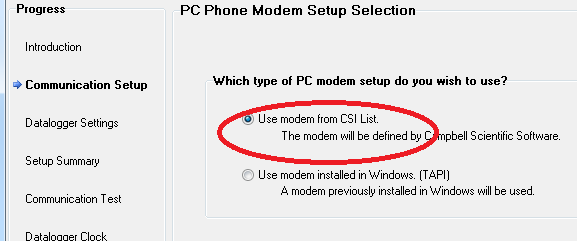
\includegraphics[width=320pt]{images/modem2}
        \caption{Seleccionar puerto}
        \label{modem2}
\end{figure}
\newpage

\begin{figure}[h!]
        \centering
        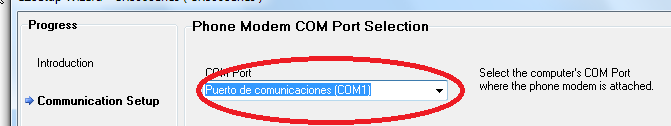
\includegraphics[width=320pt]{images/modem3}
        \caption{Ingresar numero telefónico}
        \label{modem3}
\end{figure}
\begin{figure}[h!]
        \centering
        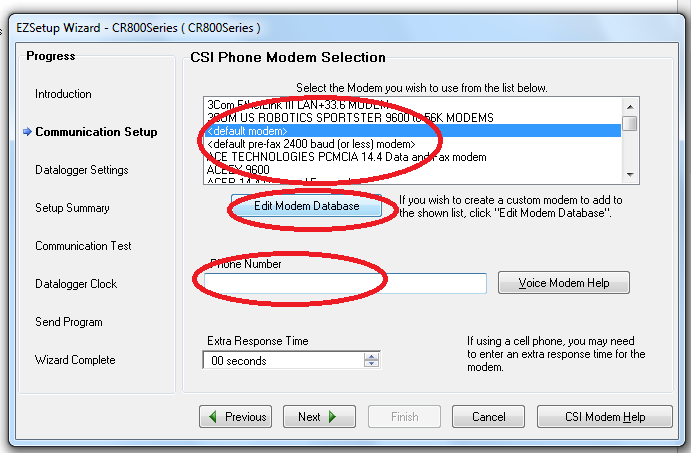
\includegraphics[width=320pt]{images/modem4}
        \caption{Agregar nuevo módem}
        \label{modem4}
\end{figure}

\newpage
\begin{figure}[h!]
        \centering
        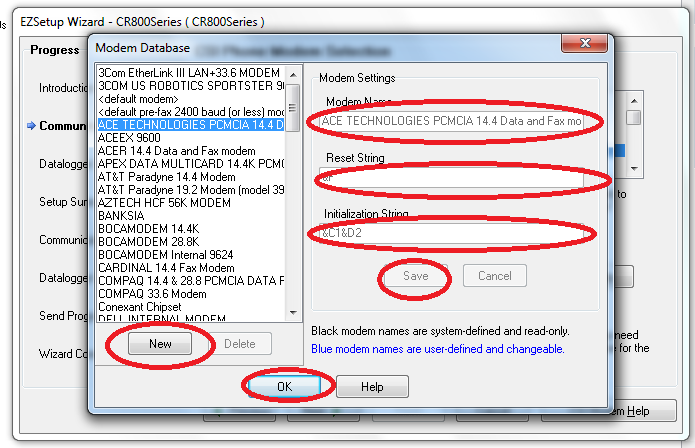
\includegraphics[width=300pt]{images/modem5}
        \caption{Ingresar dirección IP}
        \label{modem5}
\end{figure}

\newpage
\section{Verificación de datos}
Una ves desarrollado el sistema con todas las aplicaciones que cubren los requerimientos planteados en el capitulo \ref{alcances} de esta Memoria, es necesario verificar que los datos obtenidos sean correctos y de la misma forma los cálculos a los que estos son sometidos.\\
Ha quedado expresado en la sección de requerimientos que la confiabilidad de los datos así como del proceso de calculo es esencial en el funcionamiento del sistema, pequeños errores en el sistema de calculo podrían significar grandes errores en el dimensionamiento de los sistemas fotovoltaicos, lo que podría traer consecuencias poco deseables a los actores de la RedSolLAC.\\
Es necesario recordar que durante el desarrollo de esta Memoria se implementó un nuevo método de calculo, que intenta mejorar sistemas anteriores, por lo que es sumamente necesario comprobar y exponer las diferencias en los resultados obtenidos, así como de resaltar las mejoras que este método propone.\\

Los resultados obtenidos fueron comparados con diferentes fuentes de datos, así como con diferentes modelos de cálculos, algunos de ellos, los mas relevantes, son presentados a continuación junto con el análisis correspondiente a las diferencias encontradas.\\
La primera verificación apunta a comprobar que el modelo matemático haya sido bien implementado, luego se presentan 3 resultados obtenidos con la calculadora desarrollada y 2 sistemas externos, finalmente comparamos los resultados teóricos con los obtenidos en un sistema PV en operación.\\

\subsection{PVWatts}
A la fecha de desarrollo de esta Memoria, es el único software en formato Web existente, que ofrece el servicio de calculo y dimensionamiento de sistemas fotovoltaicos que cuenta con información para algunas localidades en Latinoamérica. Sin embargo en su método de calculo implementa un modelo basado en la ''media de la radiación mensual'', como consecuencia de esto, entrega resultados notablemente inferiores al real.\\ 
\subsection{PVSyst}
Es un software privativo, de uso profesional para el sector de la industria energética solar. Este software permite diseñar, estudiar, dimensionar y simular sistemas fotovoltaicos, con un método de calculo bastante complejo y cercano al funcionamiento real de una planta solar fotovoltaica, considerando complejas variables que influyen en el calculo, tales como el sombreado producido por los mimos módulos del sistema o la sombra generada por cerros cercanos a las instalaciones.\\

\subsection{Comparación ''solarCalc'' con ''Plataforma Web para sistemas térmicos''}
La ''Plataforma Web para sistemas térmicos (Ver Anexo \ref{memoriaEdu2})'' es una de las bases con las cuales se implemento el sistema de calculo. Para el proceso de verificación se utiliza una ''macro en excel'' originada en dicho trabajo y los resultados entregados en modo de depuración por la calculadora.\\
Mediante este método se pretende verificar que la implementación de la calculadora sea correcta y entregue los valores esperados.

\begin{landscape}
\begin{table}[h!]
\caption{Resultados verificación de ecuaciones macro excel}
\label{excel}
\resizebox{22cm}{!}{
\begin{tabular}{|l|c|c|c|c|c|c|c|c|c|c|c|c|c|c|c|c|c|c|c|c|c|c|c|c|c|}
        \hline
        \textbf{Resultados macro exel}&&&&&&&&&&&&&&&&&&&&&&&&&\\
        \hline
        \textbf{Hora del día}&0.5&1.5&2.5&3.5&4.5&5.5&6.5&7.5&8.5&9.5&10.5&11.5&12.5&13.5&14.5&15.5&16.5&17.5&18.5&19.5&20.5&21.5&22.5&23.5&Total\\
        \hline
        \textbf{Radiación Global Horizontal horaria}&0&0&0&0&0&20.6&203.3&421.1&650.8&862.4&1025.2&1113.7&1113.7&1025.2&862.4&650.8&421.1&203.3&20.6&0&0&0&0&0&8594.2\\
        \hline
        \textbf{Radiación Difusa Horizontal horaria}&0&0&0&0&0&5.9&51.5&95.6&135.1&167.4&190.2&202&202&190.2&167.4&135.1&95.6&51.5&5.9&0&0&0&0&0&1695.4\\
        \hline
        \textbf{Radiación Directa Horizontal horaria}&0&0&0&0&0&14.7&151.8&325.5&515.7&695.1&835&911.7&911.7&835&695.1&515.7&325.5&151.8&14.7&0&0&0&0&0&6899\\
        \hline
\end{tabular}
}
\end{table}

\begin{table}[h!]
\caption{Resultados verificación de ecuaciones calculadora}
\label{ecuacionCalc}
\resizebox{22cm}{!}{
\begin{tabular}{|l|c|c|c|c|c|c|c|c|c|c|c|c|c|c|c|c|c|c|c|c|c|c|c|c|c|}
        \hline
        \textbf{Resultados macro excel}&&&&&&&&&&&&&&&&&&&&&&&&&\\
        \hline
        \textbf{Hora del día}&0.5&1.5&2.5&3.5&4.5&5.5&6.5&7.5&8.5&9.5&10.5&11.5&12.5&13.5&14.5&15.5&16.5&17.5&18.5&19.5&20.5&21.5&22.5&23.5&Total\\
        \hline
        \textbf{Radiación Global Horizontal horaria}&0&0&0&0&0&21&204&421&651&862&1025&1114&1114&1025&862&651&421&204&21&0&0&0&0&0&8596\\
        \hline
        \textbf{Radiación Difusa Horizontal horaria}&0&0&0&0&0&6&52&96&135&167&190&202&202&190&167&135&96&52&6&0&0&0&0&0&1696\\
        \hline
        \textbf{Radiación Directa Horizontal horaria}&0&0&0&0&0&15&152&325&516&695&835&912&912&835&695&516&325&152&15&0&0&0&0&0&6900\\
        \hline
\end{tabular}
}
\end{table}
\end{landscape}

\newpage
Como se puede apreciar en las tablas \ref{excel} y \ref{ecuacionCalc} la pequeña diferencia obtenida en los resultados, solo atienden a una diferencia de aproximación numérica, mas haya de eso, los números verifican que el modelo de calculo ha quedado implementado correctamente.

\subsection{''solarCalc'' v/s ''PVWatts'' v/s ''PVSist con datos de la comuna Antofagasta}
\begin{table}[h!]
\caption{Comparación de software con datos de Antofagasta}
\resizebox{15cm}{!}{
\begin{tabular}{|c|c|c|c|c|}
        \hline
	\textbf{Mes}&\textbf{Antofagasta (kWh/m2/dia)}&\textbf{Energía estimada PVWatts (kWh)}&\textbf{Energía estimada solarCalc (kWh)}&\textbf{Energía estimada PVSist (kWh)}\\
	Ene&	7.70&	630&	794&	652\\
        \hline
	Feb&	7.62&	593&	751&	622\\
        \hline
	Mar&	6.71&	642&	797&	686\\
        \hline
	Abr&	5.48&	570&	690&	617\\
        \hline
	May&	4.12&	472&	566&	527\\
        \hline
	Jun&	3.63&	423&	505&	471\\
        \hline
	Jul&	3.75&	444&	528&	492\\
        \hline
	Ago&	4.65&	514&	528&	569\\
        \hline
	Sep&	5.68&	556&	676&	595\\
        \hline
	Oct&	6.68&	620&	755&	645\\
        \hline
	Nov&	6.96&	578&	710&	579\\
        \hline
	Dic&	7.63&	620&	777&	636\\
        \hline
	Total&5.87&	6662&	8172&	7089\\
        \hline
\end{tabular}
}
\end{table}
Tal como se aprecia en la tabla de datos, los resultados obtenidos por la ''solarCalc'' son notoriamente mas elevados que ambos sistemas, un $18\%$ mas que ''PVWatts'' y un $13\%$ mas que ''PVSyst'' estos son resultados esperados, en primer lugar, la primera diferencia se supone debido a la mejora con el método de calculo propuesto, la segunda diferencia si bien sigue siendo elevada es ligeramente menor esto se explica debido a que la calculadora a pesar de que mejora el método de calculo acercandoce mas al ideal de ''PVSyst'' no considera un parámetro sumamente importante como lo es la disminución en rendimiento por causa de la temperatura ambiente, la cual produce una significativa disminución de la producción cuando estas son elevadas como se puede espera de la zona norte de Chile.

\newpage
\subsection{''solarCalc'' v/s ''PVWatts'' v/s ''PVSist con datos de Vitacura}
\begin{table}[h!]
\caption{Comparación de software con datos de Vitacura}
\resizebox{15cm}{!}{
\begin{tabular}{|c|c|c|c|c|}
        \hline
	\textbf{Mes}&\textbf{Vitacura (kWh/m2/dia)}&\textbf{Energía estimada Pivotas (kW)}&\textbf{Energía estimada solarCalc (kWh)}&\textbf{Energía estimada PVSist (kWh)}\\
	Ene&	7.6&	641&	778&	609\\
        \hline
	Feb&	7.45&	563&	751&	609\\
        \hline
	Mar&	6.39&	550&	811&	684\\
        \hline
	Abr&	4.69&	393&	665&	595\\
        \hline
	May&	3.29&	288&	537&	516\\
        \hline
	Jun&	2.75&	233&	469&	440\\
        \hline
	Jul&	2.77&	245&	464&	434\\
        \hline
	Ago&	3.81&	340&	576&	539\\
        \hline
	Sep&	4.74&	407&	604&	526\\
        \hline
	Oct&	5.6&	492&	648&	545\\
        \hline
	Nov&	7.11&	592&	725&	583\\
        \hline
	Dic&	7.09&	600&	716&	592\\
        \hline
	Total&	5.26&	5344&	7744&	6673\\
        \hline
\end{tabular}
}
\end{table}
Al igual que en el caso anterior los resultados apreciados son muy elevados, un $30\%$ mas que ''PVWatts'' y un $13\%$ mas que ''PVSyst''. la diferencia excesiva con de la primera cifra se explica debido a que el nuevo método de calculo considera parámetros como la latitud el cual afectan notoriamente de acuerdo a la posición del sol. En el segundo resultado observamos que la diferencia se mantiene con el caso de Antofagasta lo que representa una buena señal al mantener el mismo porcentaje de diferencia.

\newpage
\subsection{''solarCalc'' v/s ''PVWatts'' v/s ''PVSist con datos de Concepción}
\begin{table}[h!]
\caption{Comparación de software con datos de Concepción}
\resizebox{15cm}{!}{
\begin{tabular}{|c|c|c|c|c|}
        \hline
	\textbf{Mes}&\textbf{Concepción (kWh/m2/día)}&\textbf{Energía estimada PVWatts (kWh)}&\textbf{Energía estimada solarCalc (kWh)}&\textbf{Energía estimada PVSist (kWh)}\\
	Ene&	7.64&	662&	778&	628\\
        \hline
	Feb&	6.81&	574&	751&	603\\
        \hline
	Mar&	4.93&	511&	811&	639\\
        \hline
	Abr&	3.39&	381&	665&	575\\
        \hline
	May&	1.89&	218&	537&	375\\
        \hline
	Jun&	1.54&	180&	469&	327\\
        \hline
	Jul&	1.79&	220&	464&	405\\
        \hline
	Ago&	2.53&	292&	576&	460\\
        \hline
	Sep&	3.97&	422&	604&	557\\
        \hline
	Oct&	5.42&	530&	648&	593\\
        \hline
	Nov&	6.55&	568&	725&	557\\
        \hline
	Dic&	7.54&	641&	716&	597\\
        \hline
	Total&	4.49&	5198&	7744&	6315\\
        \hline
\end{tabular}
}
\end{table}
Finalmente la ultima comparación realizada, es para la comuna de Concepción. Los resultados obtenidos fueron de un $18\%$ para ''PVWatts'' y $0,32\%$ para ''PVSyst''. Analizando estos resultados se puede concluir que son muy favorables ya que en primer lugar mantenemos la mejora con respecto del primer sistema y por otro lado nos acercarnos de manera muy precisa al software de simulación profesional. Lo importante de este resultado es que la comparación con ''PVSyst'' es muy buena y esto se explica ya que en el sur del país las temperaturas promedio durante la hora de funcionamiento de las plantas son notoriamente menores que en Antofagasta y Santiago, esto viene a corroborar la tesis donde se plantea que la corrección por temperatura de la que carece la calculadora afectan significativamente a los cálculos.

\newpage
\subsection{Comparación con sistema PV en operación}
La ultima verificación a la cual se ha sometido la aplicación construida es una verificación empírica. Utilizando un sistema fotovoltaico en operación (Ver Cap \ref{alcances}), se ha obtenido una muestra para el mes de Septiembre 2012, luego esta muestra se ha comparado con la simulación entregada por ''solarCalc'' y por ''PVSyst''. Si bien la muestra obtenida es en un periodo bastante corto como para concluir de manera definitiva sobre la correctitud del sistema, es una muestra que nos da una aproximación respecto de que tan cerca puede estar el resultado teórico con el resultado obtenido en la planta real.\\

\begin{table}
\caption{Comparación de resultados teóricos v/s empíricos para el mes de Septiembre 2012 (KWh)}
\centering
\begin{tabular}{|c|c|c|}
        \hline
        \textbf{MarceloMena}&\textbf{PVSyst}&\textbf{SolarCalc}\\
        163,4&    164,8&   190\\
        \hline
\end{tabular}
\end{table}

En los resultados obtenidos se pueden apreciar varias cosas, primeramente la similitud de los resultados entre la planta solar y ''PVSyst'' lo que nos da una idea de lo certera que es esta herramienta para el calculo y dimensionamiento de plantas solares obteniendo aproximadamente un 1\% de diferencia. Por otro lado podemos apreciar el resultado entregado por la calculadora de $190 [kWh]$ lo que representa un 16\% mas de la producción real, si bien el resultado es excesivamente alto, es un resultado sumamente esperado debido a que la calculadora no considera en su sistema de calculo la variabilidad que existe por consecuencia de la baja en el rendimiento por temperatura de operación del sistema PV.

